\documentclass[a4paper, 12pt]{article}

\usepackage[T2A]{fontenc}
\usepackage[utf8]{inputenc}
\usepackage[english,russian]{babel} %локализация
\usepackage{graphicx}%Вставка картинок правильная
\usepackage{float}%"Плавающие" картинки
\usepackage{wrapfig}%Обтекание фигур (таблиц, картинок и прочего)
\usepackage{fancybox,fancyhdr} %колонтитулы
\usepackage{amsmath, amsfonts, amssymb, amsthm, mathtools} %математика
\usepackage[left=2cm,right=2cm,
    top=2cm,bottom=2cm,bindingoffset=0cm]{geometry}
%\usepackage[12pt]{extsizes} % размер шрифта

%\documentclass[a4paper]{article}
\usepackage[14pt]{extsizes}
\usepackage[T2A]{fontenc}
\usepackage[utf8]{inputenc}
\usepackage[russian]{babel}
\usepackage{setspace,amsmath}
\usepackage{graphicx}
\usepackage{epigraph} 
\usepackage{csquotes} 
\usepackage[unicode, pdftex, hidelinks]{hyperref} 
\usepackage{amssymb} 
\usepackage{caption}
\usepackage{amsthm} 
\usepackage{float}
\usepackage{wrapfig}
\usepackage{multirow}
\usepackage[left=15mm, top=10mm, right=10mm, bottom=15mm, nohead, footskip=10mm]{geometry} 
%\pagestyle{fancy}
\newtheorem*{theorem}{\sc{Theorem}}
\newtheorem*{definition}{\sc{Definition}}
\newtheorem*{proposition}{\sc{Proposition}}
\newtheorem*{corollary}{\sc{Corollary}}
\newtheorem*{claim}{\sc{Claim}}
\newtheorem*{properties}{\sc{Properties}}
\newtheorem*{remark}{\sc{Remark}}
\DeclareMathOperator{\N}{\mathbb{N}}
\DeclareMathOperator{\Z}{\mathbb{Z}}
\DeclareMathOperator{\Q}{\mathbb{Q}}
\DeclareMathOperator{\R}{\mathbb{R}}
\RequirePackage{caption}
\DeclareCaptionLabelSeparator{d}{}
\captionsetup{justification=centering,labelsep=d}


%% Перенос знаков в формулах (по Львовскому)
\newcommand*{\hm}[1]{#1\nobreak\discretionary{}
{\hbox{$\mathsurround=0pt #1$}}{}}


\author{Вологин В. В.}

\title{Квантовая теория теплоёмкости \\ Вопрос по выбору}



\date{\today}

\begin{document}

\maketitle
\newpage

\tableofcontents{}
\newpage

\section{Введение}

Сравнение результатов классической теории теплоёмкости с эксперементальными данными показывает, что
правильно описан только определённый круг явлений. Многие явления она не объясняет
и ряд опытных фактов находится в резком противоречии с этой теорией. Например, классическая
теория не даёт объяснения зависимости теплоёмкости от температуры и даёт неправильную оценку (в
несколько раз) реальной теплоёмкости некоторых веществ при низких температурах. Также эта теория
использует довольно непоследовательный подход к подсчёту степеней свобод. Однако все трудности
такого рода были преодолены после того как теория теплоёмкости была построена на квантовой основе.


\section{Цель работы}
Сравнить прогнозы на теплоёмкости, даваемые классической и квантовой теориями. Сравнить эти
результаты с экспериментальными данными.



\section{Основная часть}
Рассмотрим различия между квантовой и классической теориями теплоёмкости на примерах двухатомного газа и кристаллической решётки металла.



\subsection{Двухатомный газ}
Рассмотрим модель двухатомного газа, например $H_2$.

\subsubsection{Классическая теория}

Согласно принципу равнораспределённости энергии по степеням свободы классическая теория теплоёмкости даёт не зависящее от T значение изохорной теплоёмкости водорода равное:

\[C_v = \frac{5}{2} R\]

Здесь считается, что молекула водорода обладает 5 степенями свободы (3 пространственные и 2 вращательные степени свободы)
А если подойти к расчёту колличества степеней свободы более основательно и учесть, что атомы не
являются материальными точками, то выяснится, что каждый из атомов водорода обладает 6 степенями свободы, а молекула и всеми 12-ю. Им соответствует средняя энергия $\frac{12}{2} kT = 6kT$. А если учесть
ещё и среднюю потенциальную энергию колебаний атомов вдоль оси ( $\frac{kT}{2}$
), то получим что молярная
изохорная теплоёмкость водорода равна:

\[C_v = \frac{13}{2} R\]

Сравнивая эти значения с даннымми, полученными экспериментально, обнаружим, что значения
теплоёмкости расходятся с реальными при любой стратегии подсчёта степеней свободы. Прежде всего
видно, что экспериментальная теплоёмкость водорода возрастает с ростом температуры, когда классическая теория теплоёмкости предсказывает её постоянной при любой температуре.

\subsubsection{Квантовая теория}
Рассмотрим наконец предложенную Эйнштейном модель, иллюстрирующую включение колебательных
степеней свободы по мере роста температуры.
Двухатомную молекулу при не слишком больших энергиях можно рассматривать как одномерный гармонический осциллятор. Не вдаваясь в тонкости квантовой механики скажем, что энергия гармонического осциллятора с циклической частотой ω может принимать только дискретный набор значений.

\begin{equation}
    \varepsilon_n = (n + \frac{1}{2} \hbar w), n = 1, 2, 3, ...    
\end{equation}

В соответствии с распределением Гиббса вероятность того, что молекула обладает энергией $\varepsilon_n$ равна:

\begin{equation}
    w_n = \frac{1}{Z} exp(- \frac{\varepsilon_n}{kT})
\end{equation}

Посчитаем стат. сумму, используя (1):

\begin{equation}
    Z = \sum_{n = 0}^{\infty}  exp(- \frac{\varepsilon_n}{kT}) = exp(- \frac{\hbar w}{2kT}) \sum_{n = 0}^{\infty}  exp(- \frac{n \hbar w}{kT}) = 
    \frac{ exp(- \frac{\hbar w}{2kT})}{1 -  exp(- \frac{\hbar w}{kT})}
\end{equation}

Зная (2) можно найти среднюю энергию молекулы:

\begin{equation}

\[    \Tilde{\varepsilon} = \sum_{n = 0}^{\infty} \varepsilon_n w_n = -\frac{\partial(ln Z)}{\partial T} = - \frac{\partial}{\partial T} [ - \frac{\hbar w}{2kT} - ln (1 - exp(- \frac{\hbar w}{kT} )] = \frac{1}{2} \hbar w \hspace{3} \cdot \hspace{3} cth(\frac{\hbar w }{2kT}) \]
\end{equation}

И тогда энергия одного моля молекул составит:
\[\Tilde{E} = \N_{A} \Tilde{\varepsilon}\]

И мы получим выражение для вклада в теплоёмкость одного моля молекул от 1 колебательной
степени свободы:

\begin{equation}
    \[ C_V = (\frac{\partial E}{\partial T})_V = R \cdot (\frac{\hbar w}{2kT})^2  \cdot \frac{1}{sh^2 (\frac{\hbar w }{2kT})}  \]
\end{equation}

Для нахождения полной молярной теплоёмкости молекулы водорода придётся учесть ещё энергии
поступательного и вращательного движения.
Говоря о вращательной энергии нужно отметить, что согласно квантовой механике роторатор (наша
линейная молекула) имеет серию вращательных уровней, энергия коорых задаётся формулой:

\[\varepsilon_{\text{вр}} = Bl(l + 1), \hspace{7} l = 1, 2, ...\]

Величина B тут называется вращательной постоянной и  связана с моментом инерции молекулы
I соотношением

\[ B = \frac{\hbar^2}{2I}\]

Согласно со сказаным выше вращаетльные степени свободы молекулы возбуждаются если температура достаточно велика: $T \gg T_{\text{вр}}$, где характеристическая температура для вращательного движения
определяется равенством
\[T_{\text{вр} } = \frac{B}{k} = \frac{\hbar^2}{2kI}\] .

В противном случае $T \ll T_{вр}$ вращательные степени свободы
остаются "замороженными".
Посчитать числовое значение суммарной молярной теплоёмкости водорода дело не простое, однако
из наших рассуждений уже понятна причина возрастания теплоёмкости водорода от температуры,
которая и проявляется в экспериментах (см рис. 1 ). Классическая теория теплоёмкости объяснения
этому явлению не даёт.

    

 \begin{figure}[H]
	\center{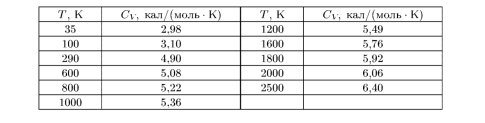
\includegraphics[scale=1.3]{Снимок.PNG} рис. 1 }
 \end{figure}


\subsection{Твёрдое тело}
Рассмотрим кристаллическую структуру. Например металл. Металл состоит из положительно заряженных ионов, совершающих тепловые колебания вокруг узлов кристалической решётки. Между ними
движутся электроны, подобно "электронному газу".

\subsubsection{Классическая теория}
Классическая теория теплоёмкости не учитывает наличие электронного газа, считая только тепловые
колебания ионов и получает достаточно близкое к правде значение:
\[C_V = 3 R \]
днако если подходить к вычислению теплоёмкости более последовательно и учесть движение электронов, приняв их за материальные точки, то теплоёмкость металов по этой теории резко возрасла бы
до неправильных значений.

\subsubsection{Квантовая теория}

В кристалле каждый атом рассматривается как трёхмерный осциллятор, совершающий колебания с
циклической частотой ω вокруг своего положения равновесия. Такой осцилятор обладает 3 колебательными степенями. Поэтому утроив результат, полученный для для двухатомного газа, получим
теплоёмкость металла:

\begin{equation}
    \[ C_V = 3 R \cdot (\frac{\hbar w}{2kT})^2  \cdot \frac{1}{sh^2 (\frac{\hbar w }{2kT})} \]
    
\end{equation}

Из полученной формулы следует что при высоких температурах ($kT \gg \hbar w$) теплоёмкость стремится
к значению $ C_V = 3R$, что согласуется с законом Дюлонга-Пти.
При низких же температурах ($kT \ll \hbar w$) теплоёмкость убывант до нуля. Сделав некоторые приближения получим что при стремлении температуры к нулю теплоёмкость убывает по следующему закону:

\[ C_V = 3 R \cdot (\frac{\hbar w}{2kT})^2  \cdot exp( - \frac{\hbar w}{kT}) \]
    
Такое поведение теплоёмкости в окреснтости нуля температуры имеет следующее физическое объяснение:
Всему виной дискретность энергетических уровней осциллятора. Просто при высоких температурах ($kT \gg \hbar w$) дискретность не проявляется, поскольку в диапазон значений энергии $\sim \hspace{2} kT$ попадает
большое колличество энергетических уровней осциллятора (рис 2a). Поэтому система и ведёт себя как
классическая. А при низких температурах kT становится сравнимо с $\hbar w   $, а после и вовсе становится
меньше расстояния между энергетическими уровнями (рис 2б). В результате лишь малая часть молекул  $\sim exp( - \frac{\hbar w}{kT}).$


 \begin{figure}[H]
	\center{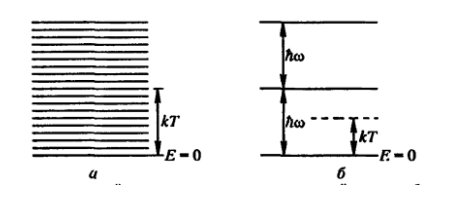
\includegraphics[scale=1.3]{ener_lev.PNG} рис. 2 }
 \end{figure}


Следует подчеркнуть что в области низких температур модель Эйнштейна передаёт поведение
теплоёмкости лишь качественно. Более точной в этом случае являетс модель Дебая, учитывающая
тот факт, что вследствие взаимодействия атомов существуют различные частоты колебаний криста␂лической решётки. согласно этой модели при низких температурах теплоёмкость убывает по закону
$C_V = \alpha T^3$ , где $\alpha = const$.
В модели теплоёмкости Эйнштейна величину $T_{\text{кол}} = \frac{\hbar w}{k}$
называют характеристической температу␂рой, определяющей условие возбуждение колебательных степеней свободы: при $T \gg T_{\text{кол}}$ колебатель␂ные степени свободы активны, а при $T \ll T_{\text{кол}}$ эти степени свободы "заморожены".
В соответсвии со сказанным выше для газов в типичных ситуациях $T_{\text{вр}} \sim 10^2K$, $T_{\text{кол}} \sim 10^3K$. Для
твёрдого тела характеристическая температура Tкол определяет условия возбуждения колебатель␂ных степеней свободы и называется температурой Дебая, а её значение обычно принадлежит интервалу
от $10^2$ K до $10^3$ К.


\subsubsection{Опытные данные}

Опытные данные для зависимости молярной изохорной теплоёмкости меди от температуры (рис. 3):

 \begin{figure}[H]
	\center{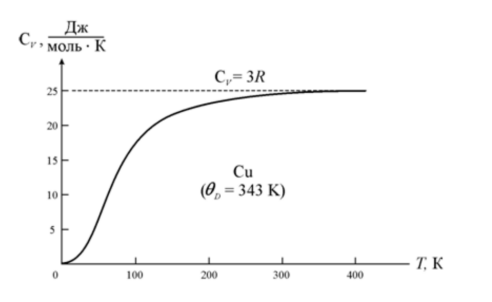
\includegraphics[scale=1.3]{exp.PNG} рис. 3 }
 \end{figure}


Как видно на больших температурах правильную оценку теплоёмкости $\sim 3R$ дают и классическая
и квантовая теории теплоёмкости. Главное отличие классической теории от реальности проявляется
при низких температурах, когда теплоёмкость металла убывает до 0, как и предсказывала теория
Эйнштейна.

\section{Выводы}

Сравнив классическую теорию теплоёмкости с кантовой теорией Эйнштейна и приложив эти данные
к реальным значениям теплоёмкостей можно прийти к выводу, что классическая теория теплоёмкости
достаточно точно оценивает значения теплоёмкости в средних и высоких диапазонах температур, когда
все степени свободы вещества разморожены, но не применима к низким температурам, на которых
теплоёмкость вещества активно возрастает. Квантовая же теория Не имеет такого недостатка и точно
оценивает поведения теплоёмкости при температурах бликих к 0, однако расчёт теплоёмкостей по этой
теории намного сложнее.

\section{Используемая литература}
1. Л.Д.Ландау, Е.М.Лившиц "Статистическая физика. Часть 1"  \newline
2. Н.А.Кириченко "Термодинамика, статистическая и молекулярная физика" \newline
3. Д.В.Сивухин "Общий курс физики. термодинамика и молекулярная физика" \newline
4. В. А. Гуртов Р. Н. Осауленко "Физика твёрдого тела для инженеров" \newline
\end{document}
